\section{Explicit ODE solver} \label{part2}
We consider the initial value problem
\begin{equation} \label{2_problem}
    \Dot{x}(t) = f(t,x(t),p), \hspace{1em} x(t_0) = x_0,
\end{equation}
where $x \in \mathbb{R}^{n_x}$ and $p \in \mathbb{R}^{n_p}$.

\subsection{Describe the explicit Euler algorithm (i.e. provide an algorithm for it in your report and explain how you get from the differential equations to the numerical formulas).}

Taking a solution $x(t)$ of the IVP (\ref{2_problem}), we consider its Taylor expansion around time $t_0$:
\begin{align*}
    x(t_0 + h) &= x(t_0) + hx'(t_0) + \frac{h^2}{2}x''(t_0) + \mathcal{O}(h^3) \\
    & \approx x(t_0) + hx'(t_0).
\end{align*}
By ignoring quadratic terms and noticing that $x'(t) = f(t, x(t), p)$ we get the expression of the Explicit Euler method. If we discretize time as $t_n = t_0 + n \cdot h \, : 0 \leq n \leq N$ we can calculate a mesh function $x_n$ at each point in the following way:
\begin{align*}
    x_0 &= x(t_0), \\
    x_n &= x_{n-1}  + h f(t_{n-1}, x_{n-1}, p) \hspace{1em} \text{for } n = 1, 2, \ldots, N.
\end{align*}
The numerical solution $x_n \to x(t_n)$ as $h \to 0$. This is proven by the derivation of convergence and global error order of the method in exercise \ref{1_4}.

%%%%%%%%%%%%%%%%%%%%%%%%%%%%%%%%%%%%%%%%%%%%%%%%%%%%%%%%%%%%%%%%%%%%%%%%%%%%%%%%%%%%%%%%%%%%%%%%%%%

\subsection{Implement an algorithm in Matlab for the explicit Euler method with fixed time-step and provide this in your report. Use a format that enables syntax highlighting.}
\begin{lstlisting}[caption = Explicit Euler method with fixed time step size, captionpos=b, label=2_ExEuler_fixed]
function [T,X] = EulerExplicit_fixed(fun, tspan, h, x0, args)

t0 = tspan(1);
tf = tspan(end);
T = t0:h:tf;
N = size(T,2);
X = zeros(size(x0,1), N);
X(:,1) = x0;

for k = 1:N-1
    f = feval(fun, T(k), X(:,k), args{:});
    X(:,k+1) = X(:,k) + h * f;
end
end

\end{lstlisting}

%%%%%%%%%%%%%%%%%%%%%%%%%%%%%%%%%%%%%%%%%%%%%%%%%%%%%%%%%%%%%%%%%%%%%%%%%%%%%%%%%%%%%%%%%%%%%%%%%%%

\subsection{Implement an algorithm in Matlab for the explicit Euler method with adaptive time step and error estimation using step doubling.}
In this implementation we use an asymptotic time step controller. As we are going to model problems without an analytical solution, we'll use step doubling to make an estimate of the error.

\begin{lstlisting}[caption = Explicit Euler method with adaptive time step size, captionpos=b, label=2_ExEuler_adaptive]
function [T,X,r_out,h_out,info] = EulerExplicit_adaptive(fun,tspan,h0,x0,abstol,reltol,args)

epstol = 0.8;
facmin = 0.1;
facmax = 5.0;

t0 = tspan(1);
tf = tspan(end);
t = t0;
h = h0;
x = x0;

T = t0;
X = x0;
r_out = [];
h_out = [];
info = zeros(1,4);

nfun = 0;
nstep = 0;
naccept = 0;

while t < tf
    if (t+h > tf)
        h = tf-t;
    end
    f = feval(fun,t,x,args{:});
    nfun = nfun + 1;
    AcceptStep = false;
    while ~AcceptStep
        x1 = x + h*f;
        
        hm = 0.5*h;
        tm = t + hm;
        xm = x + hm*f;
        fm = feval(fun,tm,xm,args{:});
        nfun = nfun + 1;
        x1hat = xm + hm*fm;
        
        nstep = nstep + 1;
        
        e = abs(x1hat-x1);
        r = max(e./max(abstol, abs(x1hat) .* reltol));
        AcceptStep = (r <= 1.0);
        
        if AcceptStep
            t = t+h;
            x = x1hat;
            
            T = [T,t];
            X = [X,x];
            r_out = [r_out, r];
            h_out = [h_out, h];
            naccept = naccept + 1;
        end
        
        h = max(facmin, min(sqrt(epstol/r), facmax)) * h;
    end
end

info(1) = nfun;
info(2) = nstep;
info(3) = naccept;
info(4) = nstep - naccept;

end

\end{lstlisting}

% \pagebreak

%%%%%%%%%%%%%%%%%%%%%%%%%%%%%%%%%%%%%%%%%%%%%%%%%%%%%%%%%%%%%%%%%%%%%%%%%%%%%%%%%%%%%%%%%%%%%%%%%%%

\subsection{Test your algorithms on the Van der Pol problem \texorpdfstring{($\mathbf{\mu = 1.5}$ and $\mathbf{\mu = 15}$, $\mathbf{x_0 = [1.0;1.0]}$)}{mu = 1.5 and mu = 15, x0 = [1.0;1.0]}} \label{2_4}
The IVP (\ref{2_problem}) for the Van der Pol problem will be used in the entire assignment by calling the following function:

\begin{lstlisting}[caption = Van der Pol equation, captionpos=b, label=VDP_eq]
function xdot = VanderPol(t,x,mu)
xdot = zeros(2,1);
xdot(1) = x(2);
xdot(2) = mu*(1-x(1)^2)*x(2) - x(1);
end
\end{lstlisting}

Both methods will be called simply by setting the parameters and respectively:
\begin{lstlisting}
[T,X] = EulerExplicit_fixed(@VanderPol, tspan, h, x0, args);
[T,X,r_out,h_out,info] = EulerExplicit_adaptive(@VanderPol, tspan, h0, x0, abstol, reltol, args);
\end{lstlisting}

In the following plots we can observe the results of the Explicit Euler method with fixed and adaptive step size, both solving the Van der Pol problem for a $\mu$ of $1.5$ and $15$. The solutions are plotted using different step sizes for the fixed method and different tolerances for the adaptive method. The tolerance value sets both the values of \code{abstol} and \code{reltol}.

Taking a look at the results for the fixed method in Figures \ref{2_4_fixed_mu_1_5} and \ref{2_4_fixed_mu_15}, we can spot a curious behaviour. Even though the shape of the solution for high step sizes looks alike to the real solution, there is a considerable frequency difference among them. We can also see how for $\mu=15$ the problem becomes more \textit{stiff}, thus requiring a smaller step size (values of $h \sim 0.2$ made it explode).

The same behaviours can also be observed in the results for the adaptive method in Figures \ref{2_4_adaptive_mu_1_5} and \ref{2_4_adaptive_mu_15}. These plots also show the final chosen step size per every time iteration and the measure of the relative error. Of course, when the tolerance is very fine $h \to 0$ and $r \to 0.8$, which is the chosen value of \code{epstol}. For the case when $\mu = 15$, we can also observe the increase in stiffness in these two plots. Also, we can observe how the no. of function calls and steps varies when we decrease the tolerance value in Tables \ref{2_4_adaptive_mu_1_5_table} and \ref{2_4_adaptive_mu_15_table}.

\begin{figure}[H]
    \centering
    \makebox[\textwidth][c]{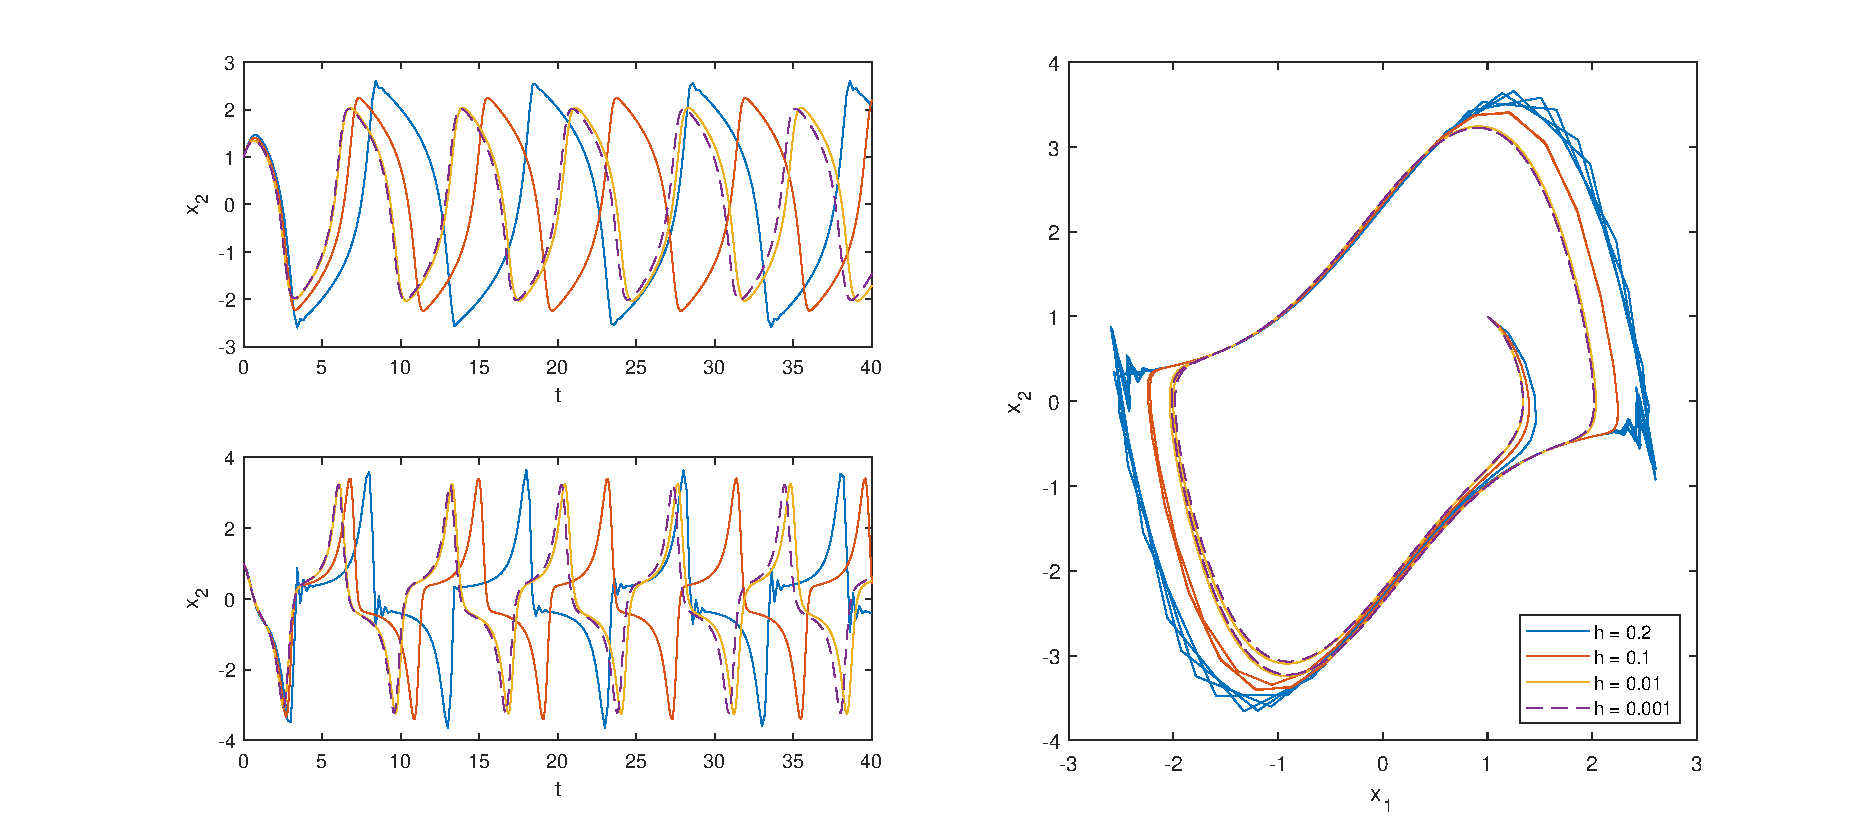
\includegraphics[width=1.25\textwidth]{images/2/2_4_fixed_mu_1_5.pdf}}
    \caption{Solution for the Van der Pol problem ($\mathit{\mu = 1.5}$) using Explicit Euler with fixed step size}
    \label{2_4_fixed_mu_1_5}
\end{figure}

\begin{figure}[H]
    \centering
    \makebox[\textwidth][c]{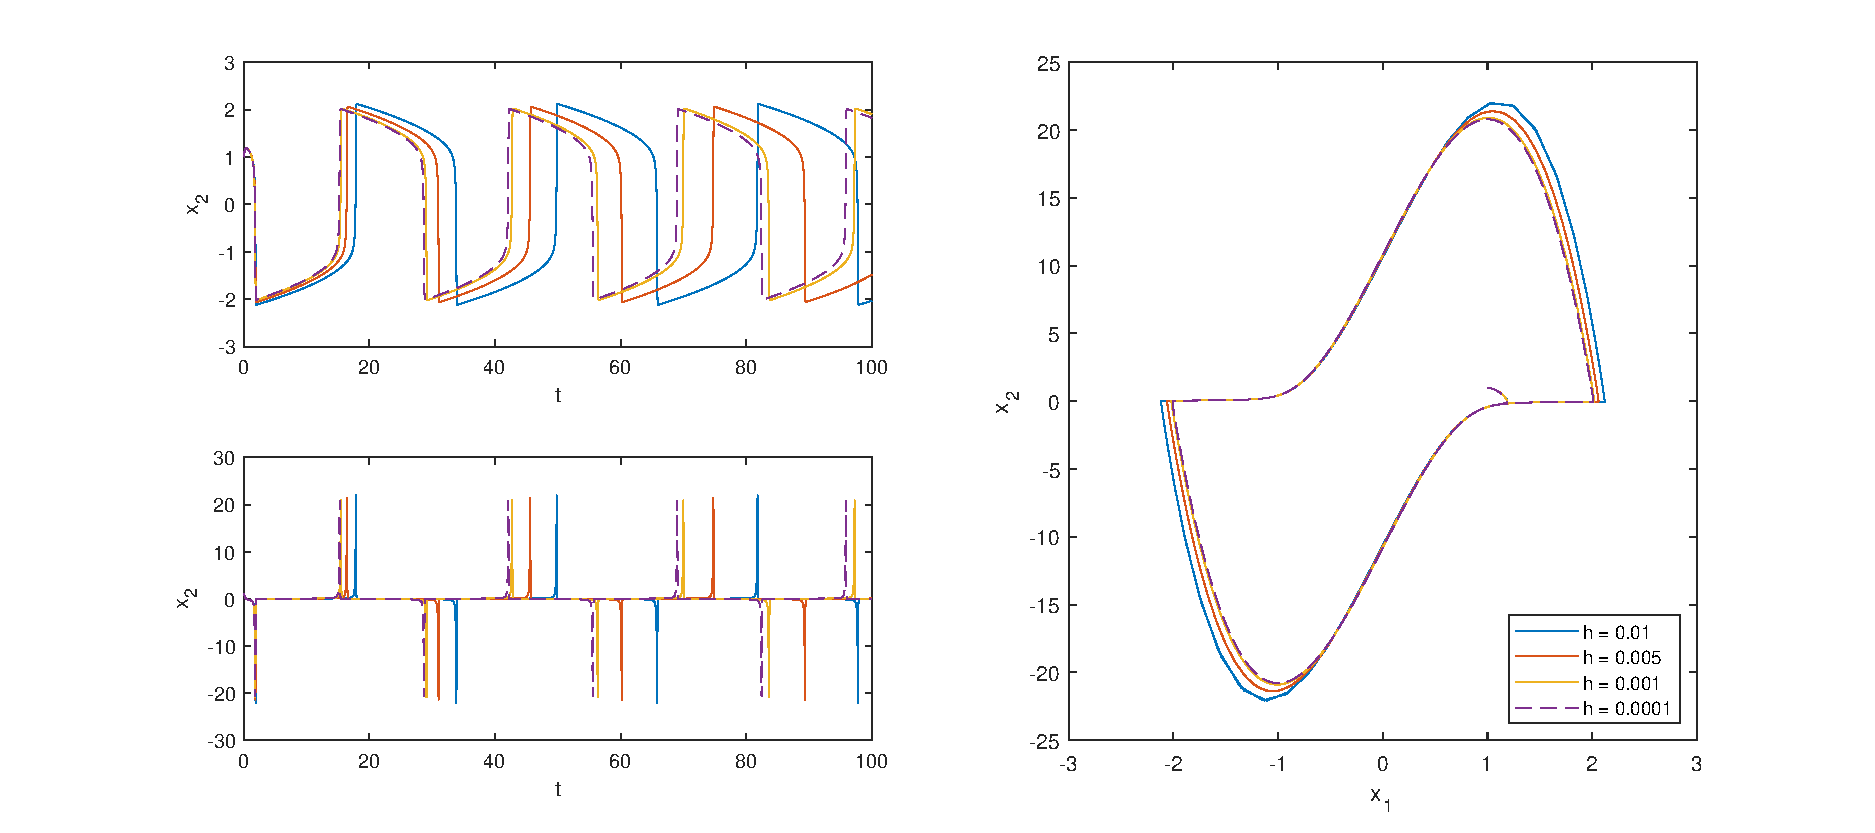
\includegraphics[width=1.25\textwidth]{images/2/2_4_fixed_mu_15.pdf}}
    \caption{Solution for the Van der Pol problem ($\mathit{\mu = 15}$) using Explicit Euler with fixed step size}
    \label{2_4_fixed_mu_15}
\end{figure}

\begin{figure}[H]
    \centering
    \makebox[\textwidth][c]{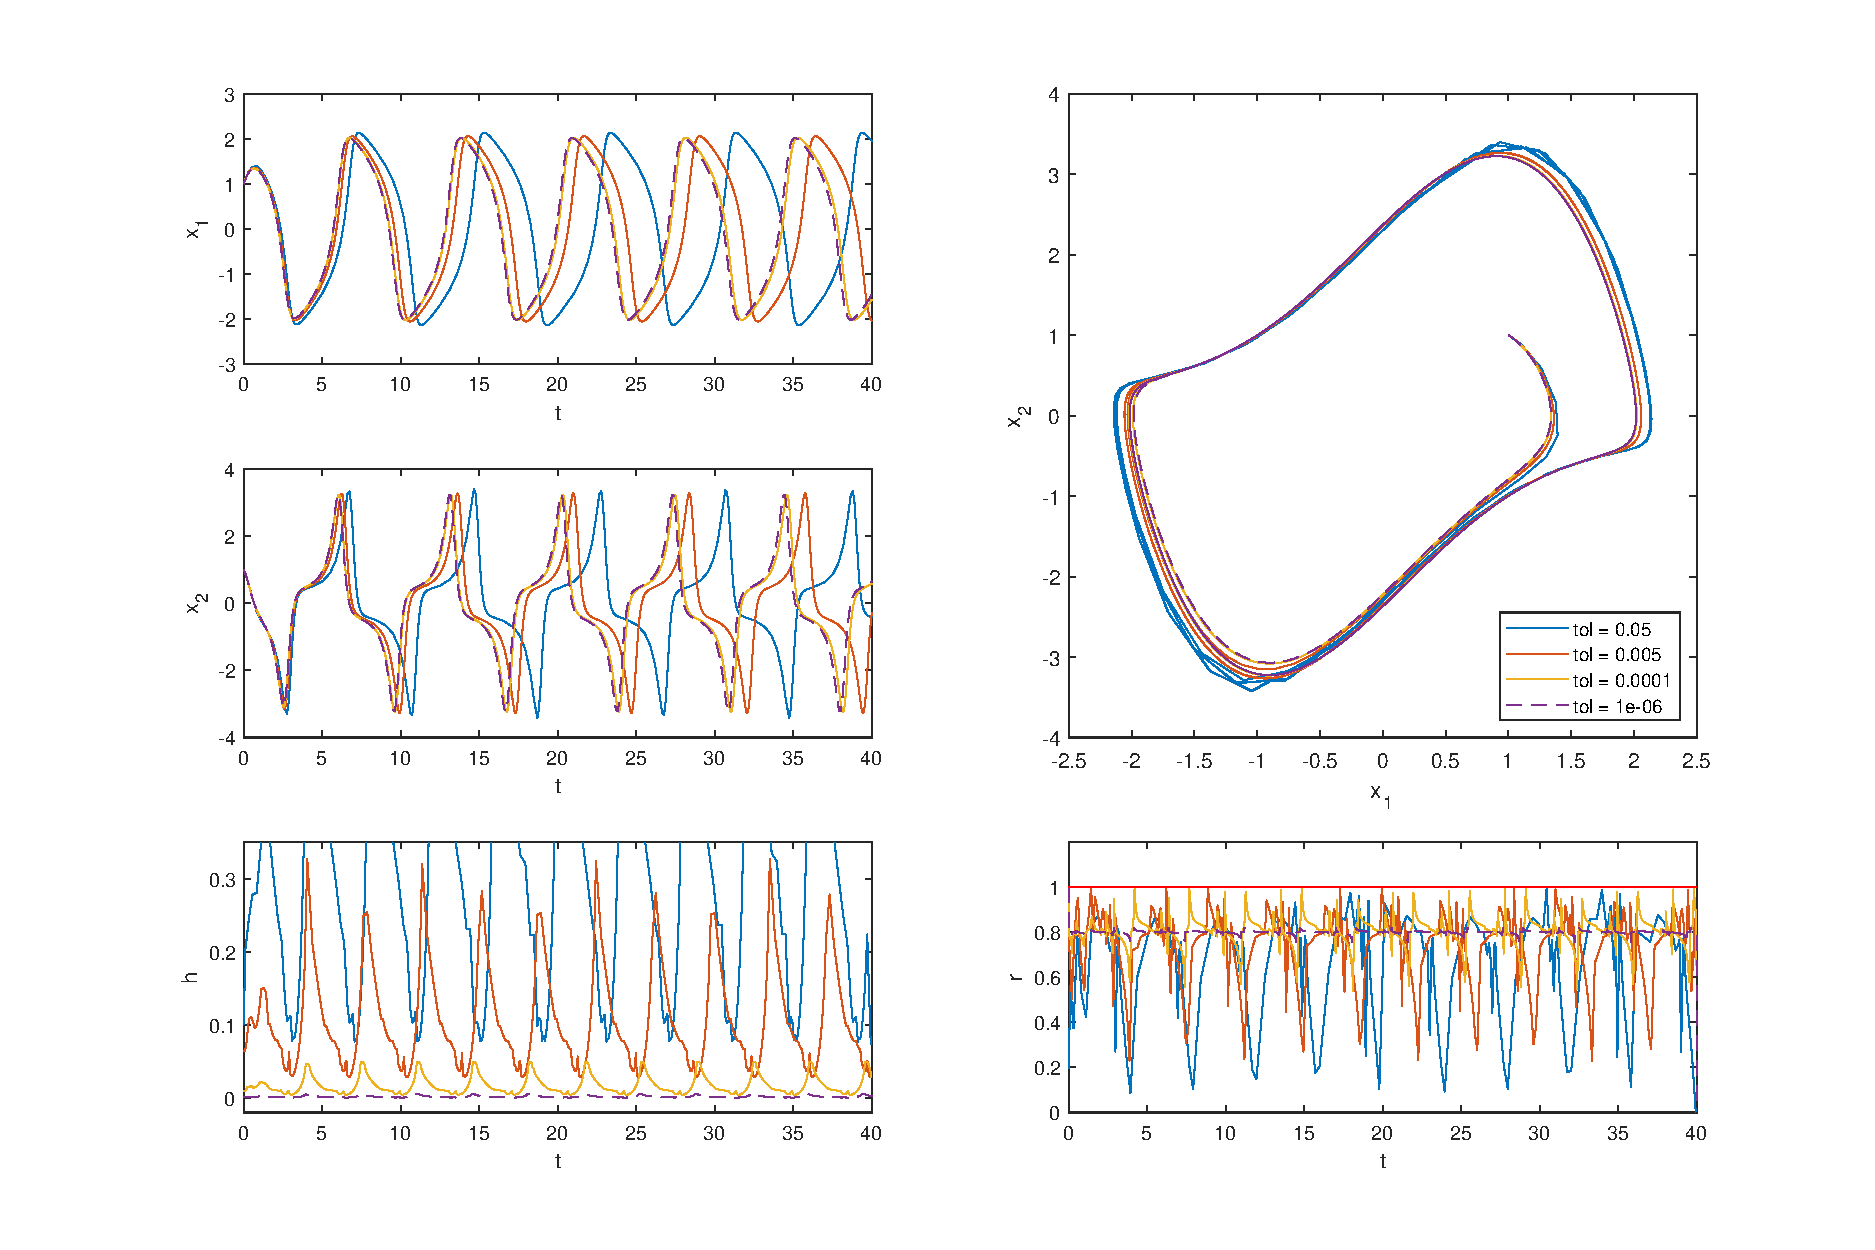
\includegraphics[width=1.25\textwidth]{images/2/2_4_adaptive_mu_1_5.pdf}}
    \caption{Solution for the Van der Pol problem ($\mathit{\mu = 1.5}$) using Explicit Euler with adaptive step size}
    \label{2_4_adaptive_mu_1_5}
\end{figure}

\begin{table}[H]
    \centering
    \begin{tabular}{@{}l|cccc@{}}
    \toprule
    Tolerances           & 0.05 & 0.005 & 0.0001 & 1e-06 \\ \midrule
    Function evaluations & 445  & 1200  & 7383   & 73678 \\
    Calculated steps     & 263  & 660   & 3695   & 36840 \\
    Accepted steps       & 182  & 540   & 3688   & 36838 \\
    Rejected steps       & 81   & 120   & 7      & 2     \\ \bottomrule
    \end{tabular}
    \caption{Parameters of the Explicit Euler with adaptive step size for the Van der Pol problem ($\mathit{\mu = 1.5}$)}
    \label{2_4_adaptive_mu_1_5_table}
\end{table}

\begin{figure}[H]
    \centering
    \makebox[\textwidth][c]{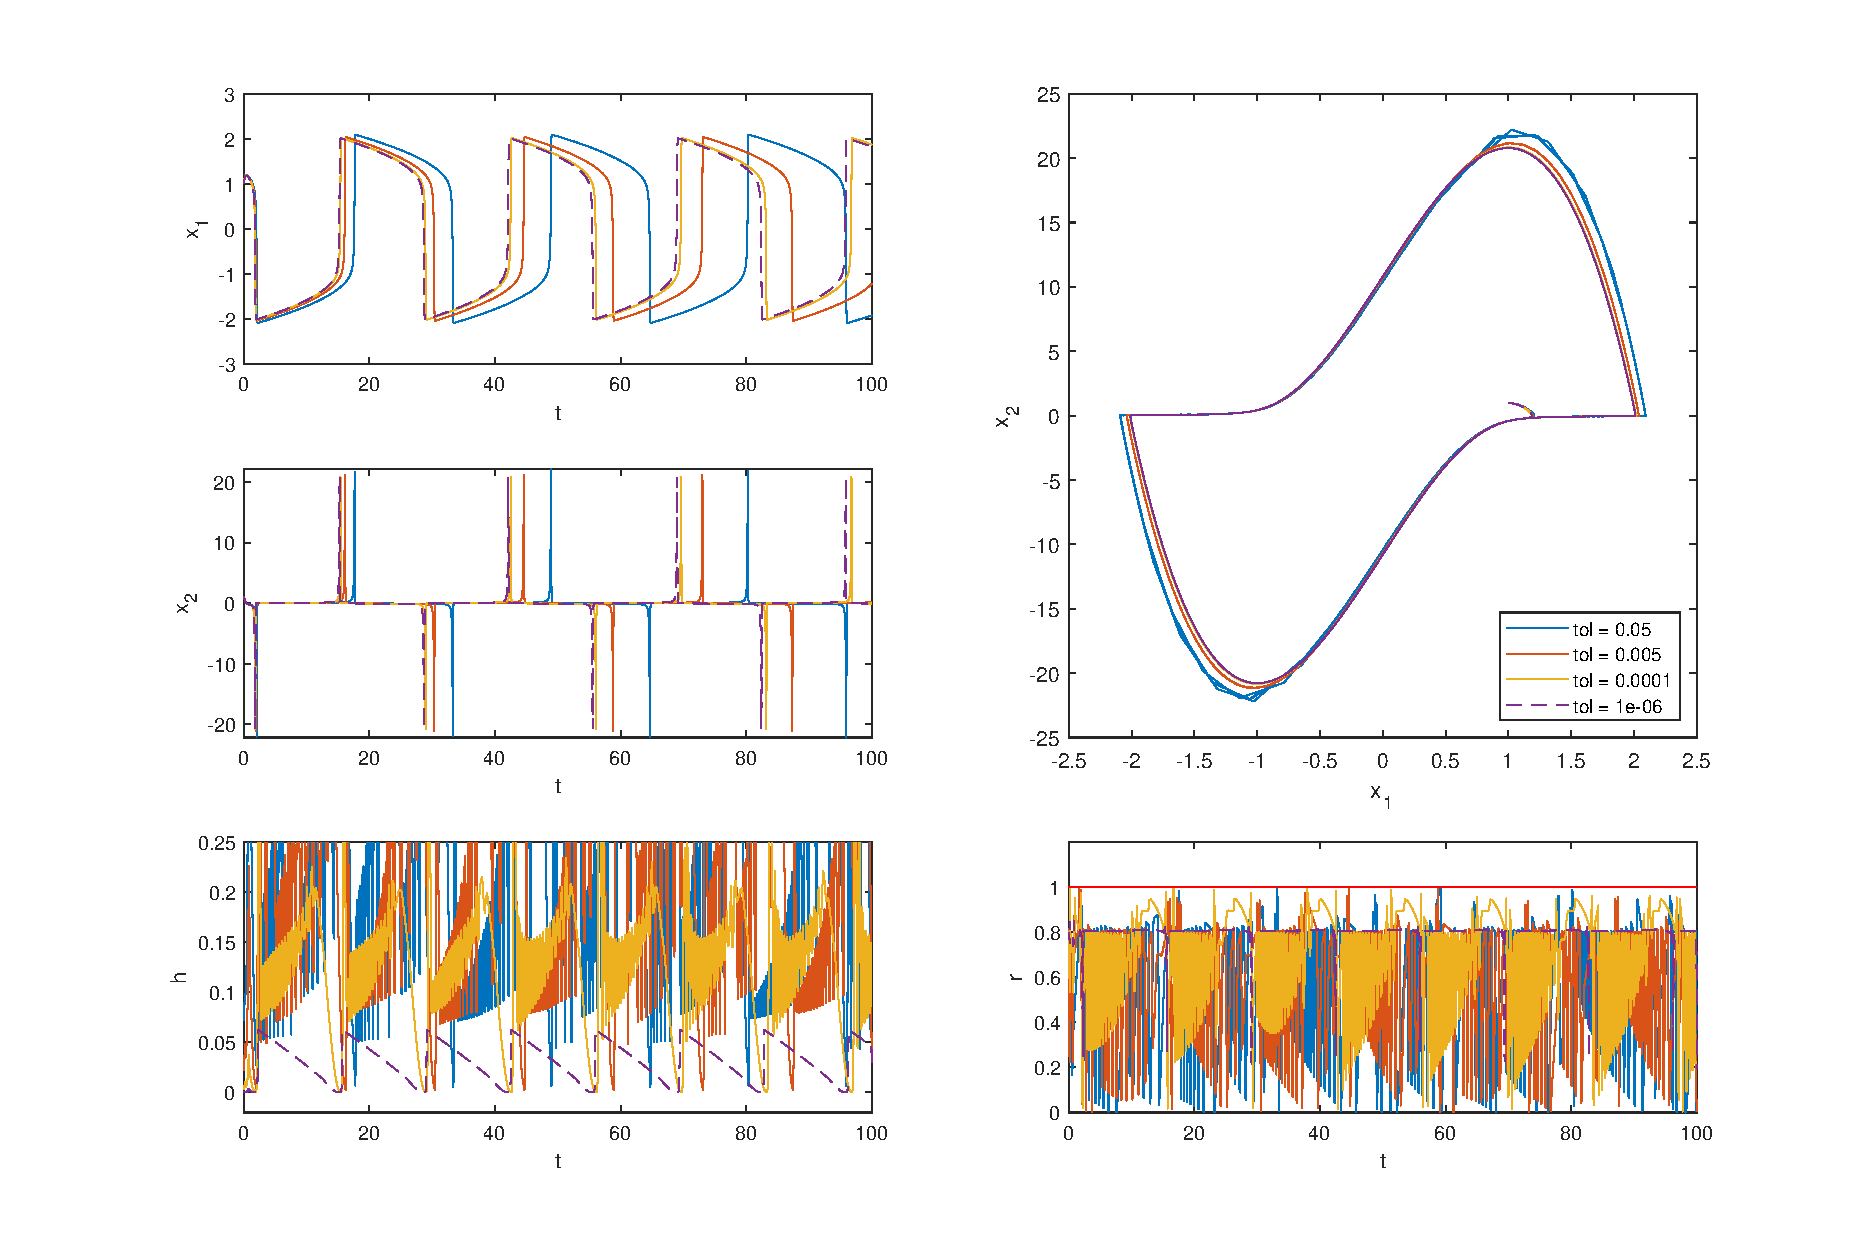
\includegraphics[width=1.25\textwidth]{images/2/2_4_adaptive_mu_15.pdf}}
    \caption{Solution for the Van der Pol problem ($\mathit{\mu = 15}$) using Explicit Euler with adaptive step size}
    \label{2_4_adaptive_mu_15}
\end{figure}

\begin{table}[H]
    \centering
    \begin{tabular}{@{}l|cccc@{}}    \toprule
    Tolerances           & 0.05 & 0.005 & 0.0001 & 1e-06      \\ \midrule
    Function evaluations & 1583 & 2485  & 11246  & 1.0404e+05 \\
    Calculated steps     & 954  & 1418  & 5740   & 52022      \\
    Accepted steps       & 629  & 1067  & 5506   & 52019      \\
    Rejected steps       & 325  & 351   & 234    & 3          \\ \bottomrule
    \end{tabular}
    \caption{Parameters of the Explicit Euler with adaptive step size for the Van der Pol problem ($\mathit{\mu = 15}$)}
    \label{2_4_adaptive_mu_15_table}
\end{table}

\pagebreak
\pagebreak
\pagebreak
\pagebreak
%%%%%%%%%%%%%%%%%%%%%%%%%%%%%%%%%%%%%%%%%%%%%%%%%%%%%%%%%%%%%%%%%%%%%%%%%%%%%%%%%%%%%%%%%%%%%%%%%%%

\subsection{Test your algorithms on the adiabatic CSTR problem described in the papers uploaded to Learn (3D-version and 1D-version).}
The IVPs (\ref{2_problem}) for both versions of the CSTR problem, obtained from \cite{Bagterp1} and \cite{Bagterp2} are included in the following functions:

\begin{lstlisting}[caption = CSTR 3D equation, captionpos=b, label=CSTR_3D_eq]
function xdot = CSTR_3D(t,x,F,params)
% F to IS units
F = F/60000;

beta = params(1);
k0 = params(2);
EaR = params(3);
CAin = params(4);
CBin = params(5);
Tin = params(6);
V = params(7);

CA = x(1);
CB = x(2);
T = x(3);
xdot = zeros(3,1);

% Rate of reaction
r = k0 * exp(-EaR/T) * CA * CB;
% Production rates and rate of temperature
RA = -r;
RB = -2*r;
RT = beta*r;
% Final ODE
xdot(1) = F/V * (CAin - CA) + RA;
xdot(2) = F/V * (CBin - CB) + RB;
xdot(3) = F/V * (Tin - T) + RT;
end

\end{lstlisting}

\begin{lstlisting}[caption = CSTR 1D equation, captionpos=b, label=CSTR_1D_eq]
function Tdot = CSTR_1D(t, T, F, params)
% F to IS units
F = F/60000;

beta = params(1);
k0 = params(2);
EaR = params(3);
CAin = params(4);
CBin = params(5);
Tin = params(6);
V = params(7);

% Rate of reaction
r = k0 * exp(-EaR/T) * (CAin + 1/beta * (Tin - T)) * (CBin + 2/beta * (Tin - T));
% Rate of temperature
RT = beta * r;
% Final ODE
Tdot = F/V*(Tin - T) + RT;
end

\end{lstlisting}

Just as in \cite{Bagterp1} and \cite{Bagterp2}, the flow will be a function of time. Its shape can be seen in Figure \ref{2_5_3D_trial}, together with a solution for the 3D-CSTR problem. The way to call the method having this flow function over time is slightly trickier than in the Van der Pol problem. I tried first creating F as a piecewise function and substituting the time in every CSTR function call. However, this was proven to be very time consuming as it implied working with symbolic functions. The best way of achieving the same output was by:
\pagebreak
\begin{lstlisting}
% Piecewise flow definition
tspans = [[0,3];[3,5];[5,7];[7,9];[9,12];[12,16];[16,18];...
    [18,20];[20,22];[22,24];[24,28];[28,32];[32,35]];
Fs = [700,600,500,400,300,200,300,400,500,600,700,200,700];

T = [];
X = [];

for i=1:size(Fs,2)
    tspan = tspans(i,:)*60;
    F = Fs(i);
    args = {F, [beta,k0,EaR,CAin,CBin,Tin,V]};
    [T_local,X_local] = EulerExplicit_fixed(@CSTR_3D, tspan, h, x0, args);
    
    T = [T, T_local(1:end-1)];
    X = [X, X_local(:,1:end-1)];
    
    x0 = X_local(:,end);
end
% Add last point and normalize
T = [T,T_local(end)]/60;
X = [X, X_local(:,end)]-273;
\end{lstlisting}

\begin{figure}[H]
    \centering
    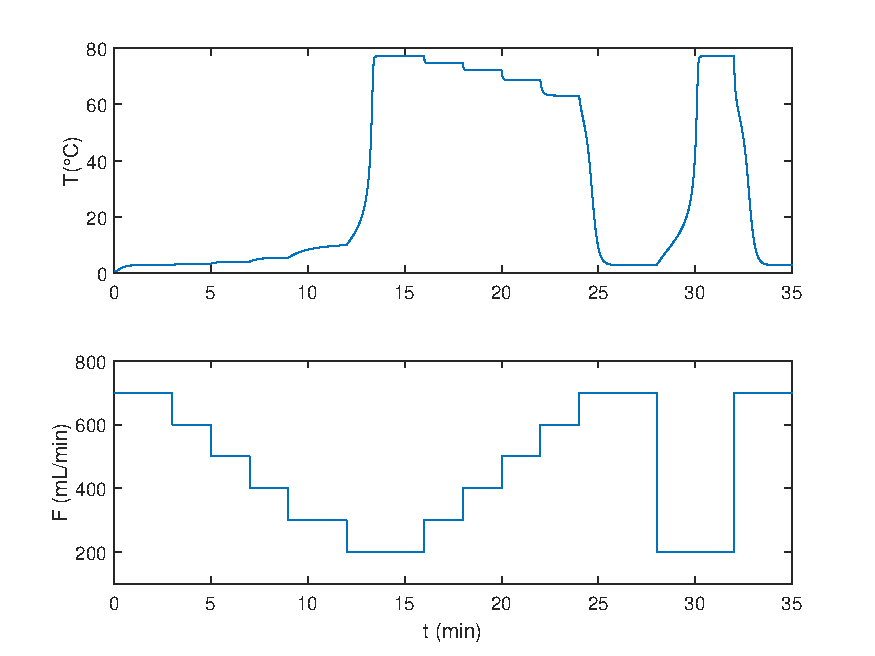
\includegraphics[width=0.8\textwidth]{images/2/2_5_3D_trial.pdf}
    \caption{Solution and value of the flow over time for the CSTR 3D problem}
    \label{2_5_3D_trial}
\end{figure}

The results for the 3D problem and 1D problem are very similar. This can be seen in Figure \ref{2_5_3D_vs_1D}, where a closeup of the interval $t \in [0,1.5]$ minutes is shown. This was the region where we can find the greatest difference between the two problems. The following plots show the results of different runs of the CSTR problems, for the fixed and adaptive Explicit Euler with different values of steps and tolerances respectively.

Taking a look at the results using the fixed method (Figure \ref{2_5_3D_1D_hs}), it's very difficult to spot a difference between the 3D and 1D case. The plot behaves the same for every chosen time step. However, the results from the adaptive in Figures \ref{2_5_3D_tols} and \ref{2_5_1D_tols} and Tables \ref{2_5_3D_tols_table} and \ref{2_5_1D_tols} are much more enlightening. In the 3D problem, the solution is pretty close even for the biggest tolerance of $0.05$. Moreover, we can observe some spike behaviour in the value of $r$ that coincides with every step change of the flow function. Also the problem becomes more stiff when the value of $F$ goes down (the r value and therefore change in h shifts a lot in these regions). This also explains the spike behaviour observed in the fixed method only at these points in time. Finally, we can observe that it takes a tighter tolerance for the 1D problem to converge. However, the number of function evaluations is a lot smaller than the 3D problem for the same tolerances and lowering down enough the tolerance yields pretty good results.

\begin{figure}[H]
    \centering
    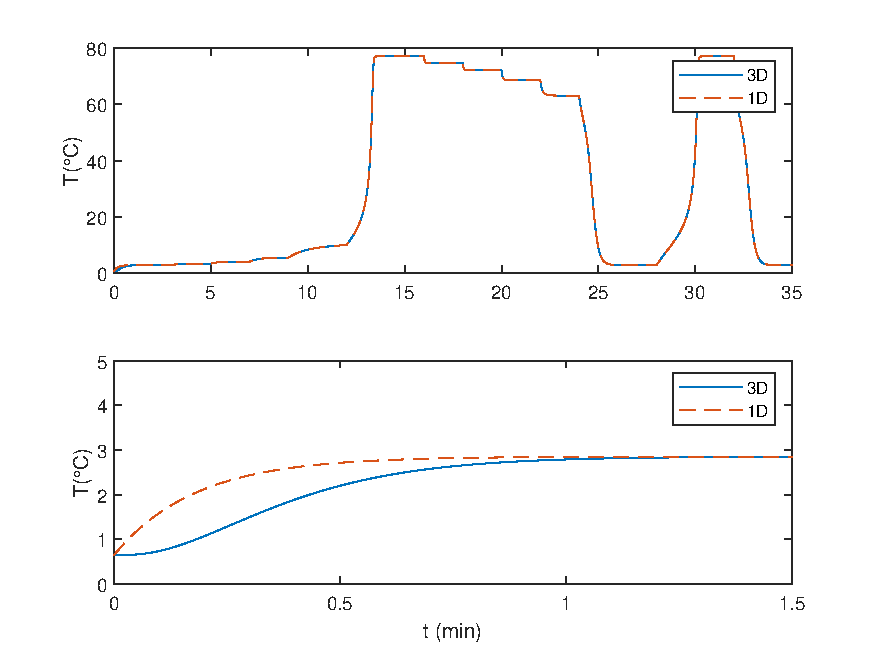
\includegraphics[width=0.8\textwidth]{images/2/2_5_3D_vs_1D.pdf}
    \caption{Comparison of the solutions for the CSTR 3D and 1D}
    \label{2_5_3D_vs_1D}
\end{figure}

\begin{figure}[H]
\centering
    \begin{subfigure}{0.8\linewidth}
        \centering
        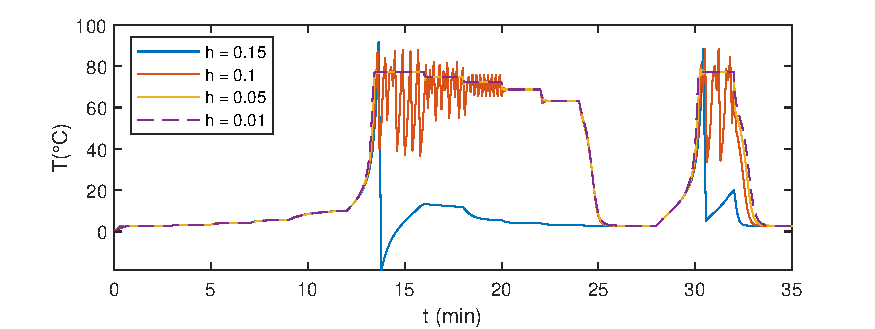
\includegraphics[width=1\linewidth]{images/2/2_5_3D_hs.pdf} 
        \caption{CSTR 3D problem}
    \end{subfigure} \\
    \begin{subfigure}{0.8\linewidth}
        \centering
        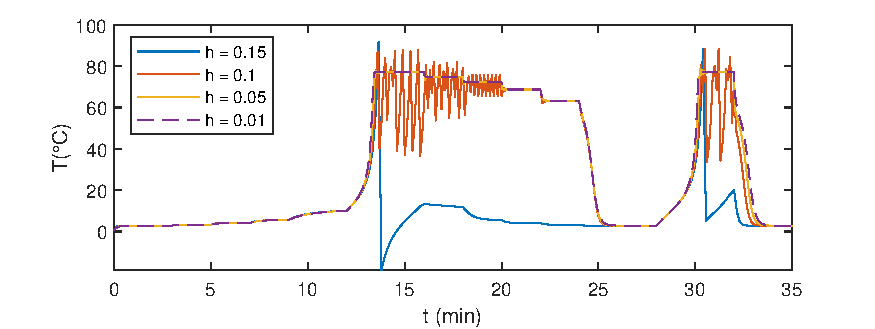
\includegraphics[width=1\linewidth]{images/2/2_5_1D_hs.pdf}
        \caption{CSTR 1D problem}
    \end{subfigure}
    \caption{Solution for the CSTR problem using Explicit Euler with fixed step size}
    \label{2_5_3D_1D_hs}
\end{figure}

\begin{figure}[H]
    \centering
    \makebox[\textwidth][c]{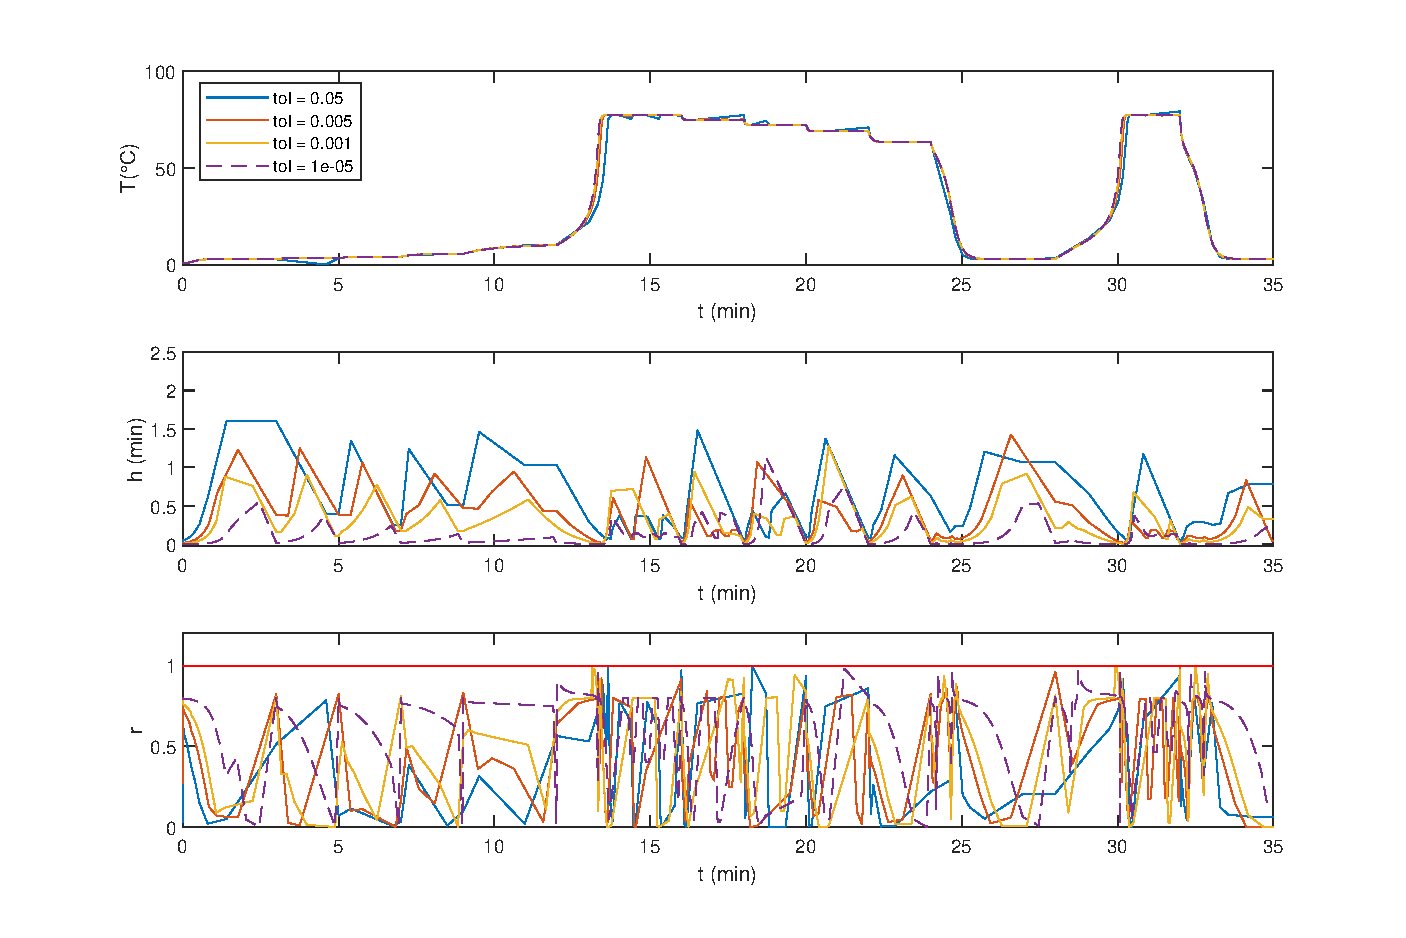
\includegraphics[width=1\textwidth]{images/2/2_5_3D_tols.pdf}}
    \caption{Solution for the CSTR 3D problem using Explicit Euler with adaptive step size}
    \label{2_5_3D_tols}
\end{figure}

\begin{table}[H]
    \centering
    \begin{tabular}{@{}l|cccc@{}}
    \toprule
    Tolerances           & 0.05 & 0.005 & 0.001 & 1e-05 \\ \midrule
    Function evaluations & 207  & 431   & 726   & 5250  \\
    Calculated steps     & 120  & 245   & 400   & 2657  \\
    Accepted steps       & 87   & 186   & 326   & 2593  \\
    Rejected steps       & 33   & 59    & 74    & 64    \\ \bottomrule
    \end{tabular}
    \caption{Parameters of the Explicit Euler with adaptive step size for the CSTR 3D problem}
    \label{2_5_3D_tols_table}
\end{table}

\begin{figure}[H]
    \centering
    \makebox[\textwidth][c]{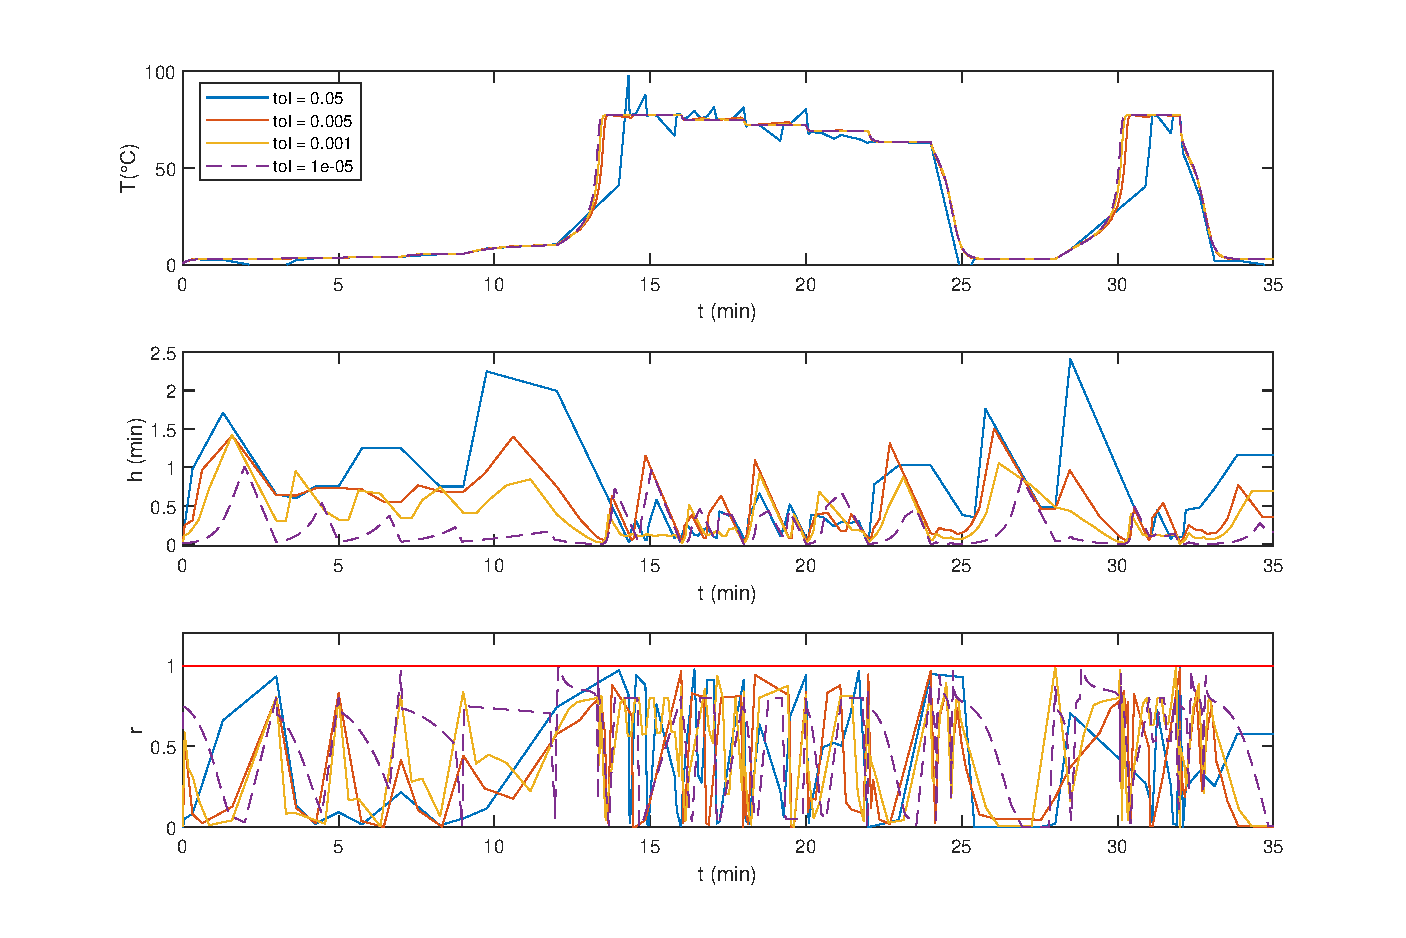
\includegraphics[width=1\textwidth]{images/2/2_5_1D_tols.pdf}}
    \caption{Solution for the CSTR 1D problem using Explicit Euler with adaptive step size}
    \label{2_5_1D_tols}
\end{figure}

\begin{table}[H]
    \centering
    \begin{tabular}{@{}l|cccc@{}}
    \toprule
    Tolerances           & 0.05 & 0.005 & 0.001 & 1e-05 \\ \midrule
    Function evaluations & 194  & 256   & 455   & 2285  \\
    Calculated steps     & 115  & 148   & 261   & 1171  \\
    Accepted steps       & 79   & 108   & 194   & 1114  \\
    Rejected steps       & 36   & 40    & 67    & 57    \\ \bottomrule
    \end{tabular}
    \caption{Parameters of the Explicit Euler with adaptive step size for the CSTR 1D problem}
    \label{2_5_1D_tols_table}
\end{table}

%%%%%%%%%%%%%%%%%%%%%%%%%%%%%%%%%%%%%%%%%%%%%%%%%%%%%%%%%%%%%%%%%%%%%%%%%%%%%%%%%%%%%%%%%%%%%%%%%%%
\pagebreak

\subsection{Compare the results from your algorithms with the results you get using some of Matlab's ODE solvers}
We'll compare the solution obtained with the explicit Euler to two ODE solvers from Matlab: \code{ode45} and \code{ode15s}. The first one is an implementation of the Dormand-Prince 5(4), a method from the Explicit Runge-Kutta family. Being an explicit method, it's not very good when dealing with stiff problems. \code{ode15s}, on the other hand, is designed to work specifically with these types of problems. Both of them are also of adaptive step size. For that reason, we will compare the Explicit Euler with adaptive step size to these two: see how they behave for a given tolerance and problem and analyse their increase in the number of function evaluations when narrowing down the tolerance.

For the Van der Pol problem, we tested Explicit Euler against \code{ode45} for the non-stiff case ($\mu = 1.5$), and against \code{ode15s} for the stiff case ($\mu = 15$). The obtained results for the Van der Pol problem (Figures \ref{2_6_mu_1_5} and \ref{2_6_mu_15} and Tables \ref{2_6_adaptive_mu_1_5_table} and \ref{2_6_adaptive_mu_15_table}) show what we discussed previously. The Explicit Euler works fine in the non-stiff case, even though the \code{ode45} achieves better accuracy with a fewer no. of function evaluations. In the stiff case, however, the no. of evaluations is ridiculously high compared to the \code{ode15s}.

\begin{figure}[H]
    \centering
    \makebox[\textwidth][c]{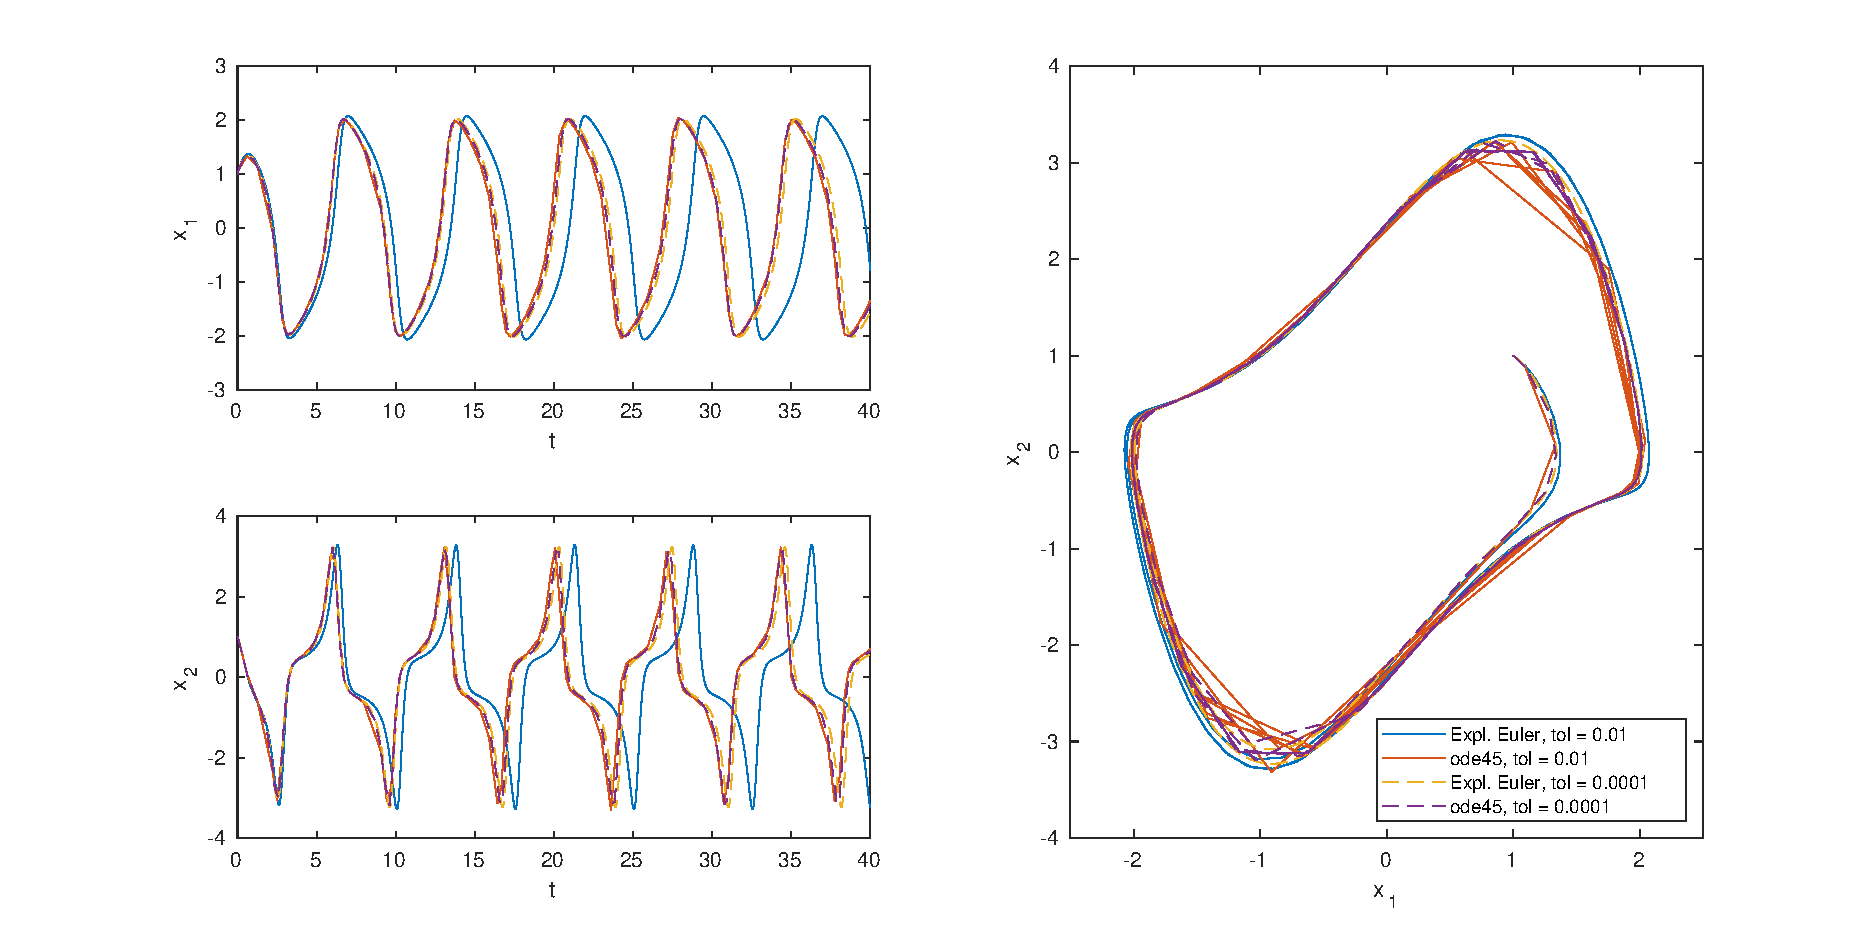
\includegraphics[width=1.25\textwidth]{images/2/2_6_mu_1_5.pdf}}
    \caption{Solution for the Van der Pol problem ($\mathit{\mu = 1.5}$) using Explicit Euler vs. \code{ode45}}
    \label{2_6_mu_1_5}
\end{figure}

\begin{table}[H]
    \centering
    \begin{tabular}{@{}l|cc|cc@{}}
    \toprule
    \textbf{Method} & \multicolumn{2}{c|}{\textbf{Expl. Euler}} & \multicolumn{2}{c}{\textbf{ode45}} \\
    Tolerances           & 0.01           & 0.0001          & 0.01       & 0.0001       \\ \midrule
    Function evaluations & 853            & 7383            & 787        & 1357         \\
    Calculated steps     & 473            & 3695            & 131        & 226          \\
    Accepted steps       & 380            & 3688            & 100        & 180          \\
    Rejected steps       & 93             & 7               & 31         & 46           \\ \bottomrule
    \end{tabular}
    \caption{Parameters of the Explicit Euler vs. \code{ode45} for the Van der Pol problem ($\mathit{\mu = 1.5}$)}
    \label{2_6_adaptive_mu_1_5_table}
\end{table}

\begin{figure}[H]
    \centering
    \makebox[\textwidth][c]{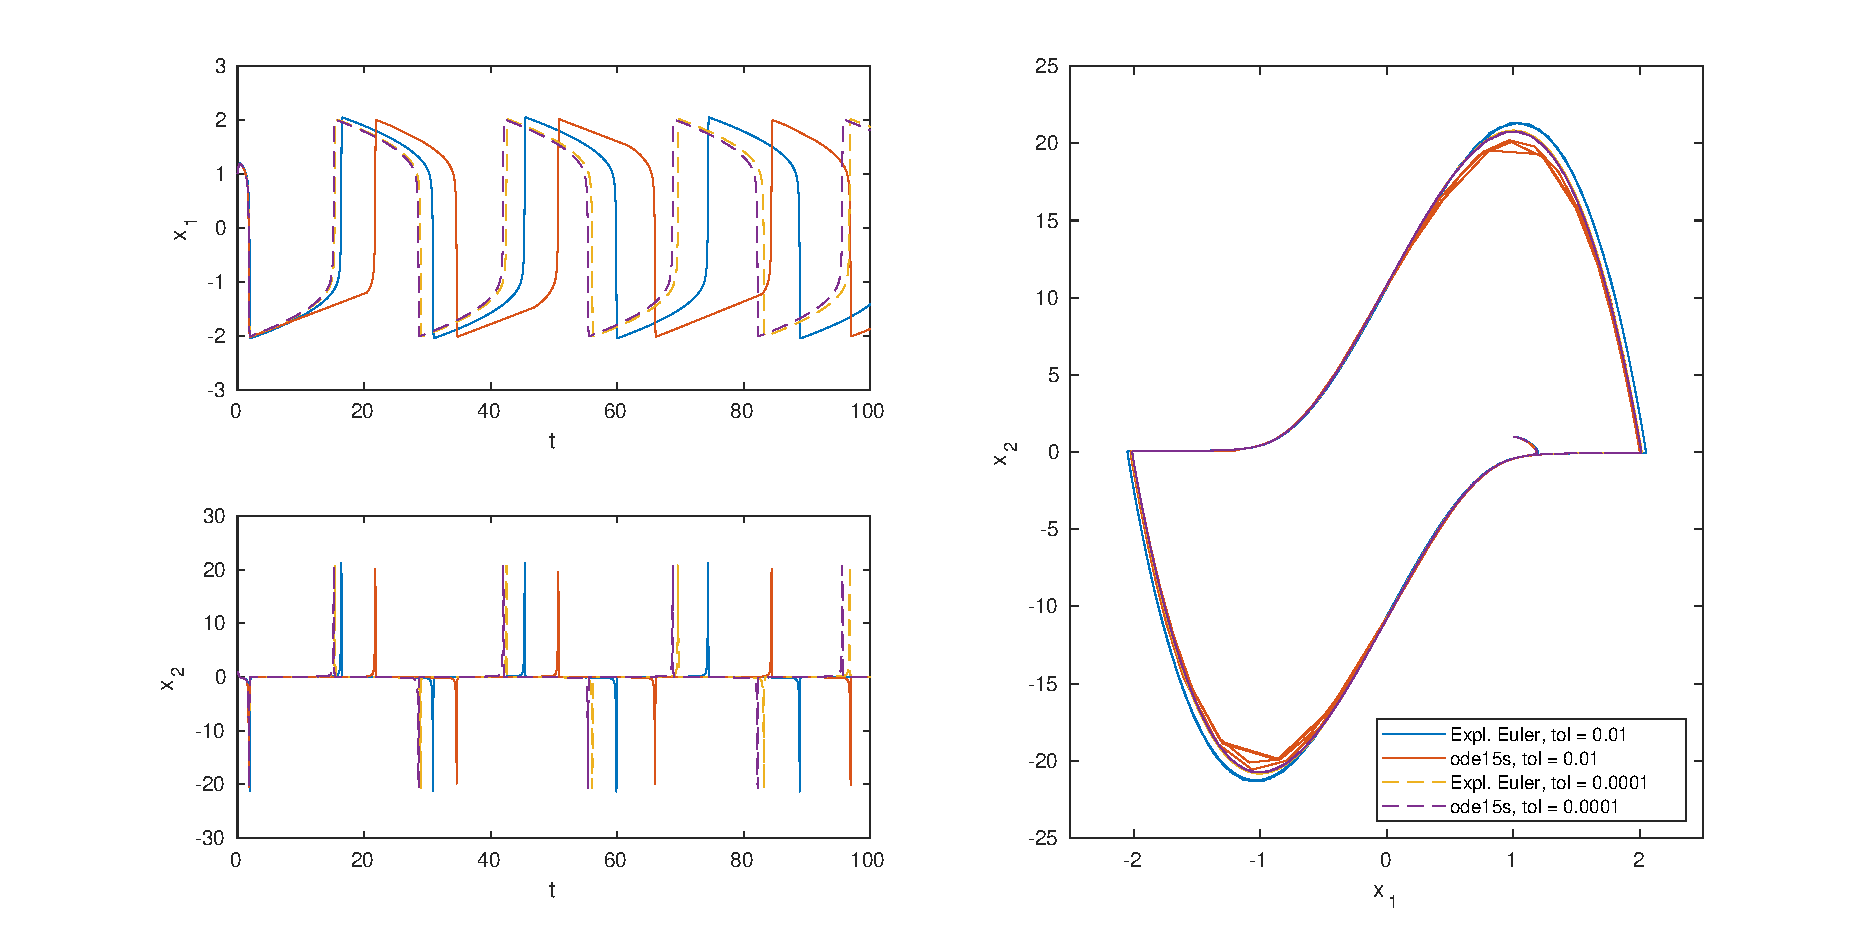
\includegraphics[width=1.25\textwidth]{images/2/2_6_mu_15.pdf}}
    \caption{Solution for the Van der Pol problem ($\mathit{\mu = 15}$) using Explicit Euler vs. \code{ode15s}}
    \label{2_6_mu_15}
\end{figure}

\begin{table}[H]
    \centering
    \begin{tabular}{@{}l|ll|ll@{}}
    \toprule
    \textbf{Method}      & \multicolumn{2}{c|}{\textbf{Expl. Euler}} & \multicolumn{2}{c}{\textbf{ode15s}} \\
    Tolerances           & 0.01               & 0.0001               & 0.01            & 0.0001            \\ \midrule
    Function evaluations & 2108               & 11246                & 1273            & 2780              \\
    Calculated steps     & 1219               & 5740                 & 558             & 1327              \\
    Accepted steps       & 889                & 5506                 & 411             & 1094              \\
    Rejected steps       & 330                & 234                  & 147             & 233               \\ \bottomrule
    \end{tabular}
    \caption{Parameters of the Explicit Euler vs. \code{ode15s} for the Van der Pol problem ($\mathit{\mu = 15}$)}
    \label{2_6_adaptive_mu_15_table}
\end{table}

For the CSTR problem, we also see how both the Explicit Euler and \code{ode45} fail where the problem turns more stiff. The \code{ode15s} achieves very good performance in this case.
\begin{figure}[H]
    \centering
    \begin{subfigure}{0.8\linewidth}
        \centering
        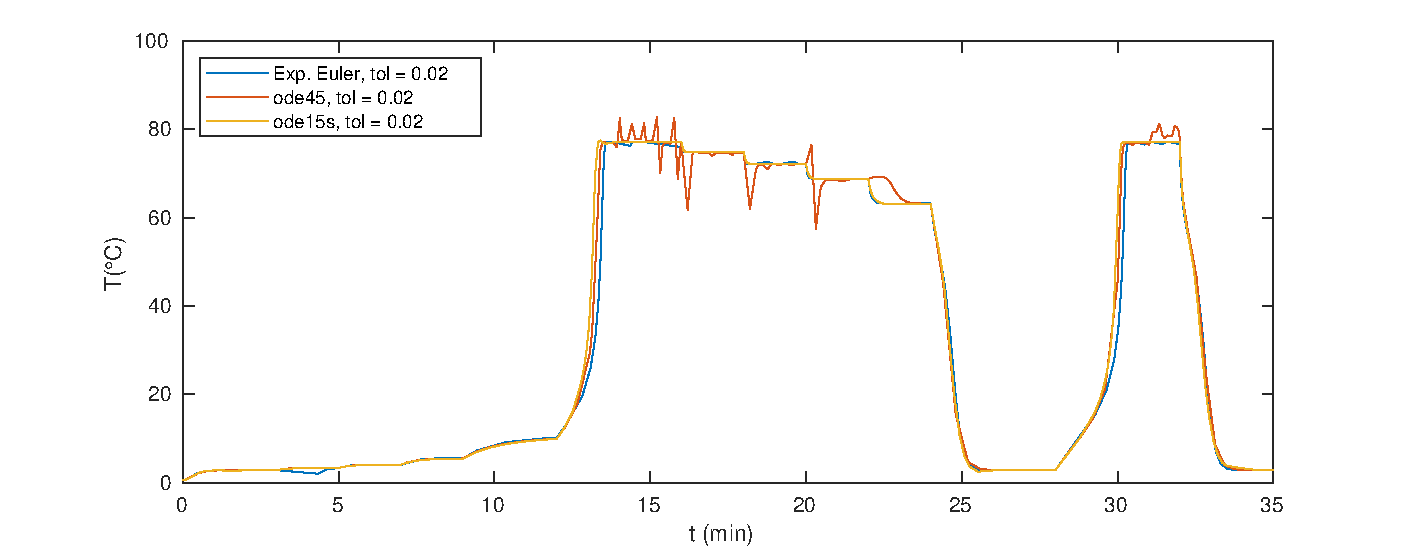
\includegraphics[width=1\linewidth]{images/2/2_6_3D.pdf} 
        \caption{CSTR 3D problem}
    \end{subfigure} \\
    \begin{subfigure}{0.8\linewidth}
        \centering
        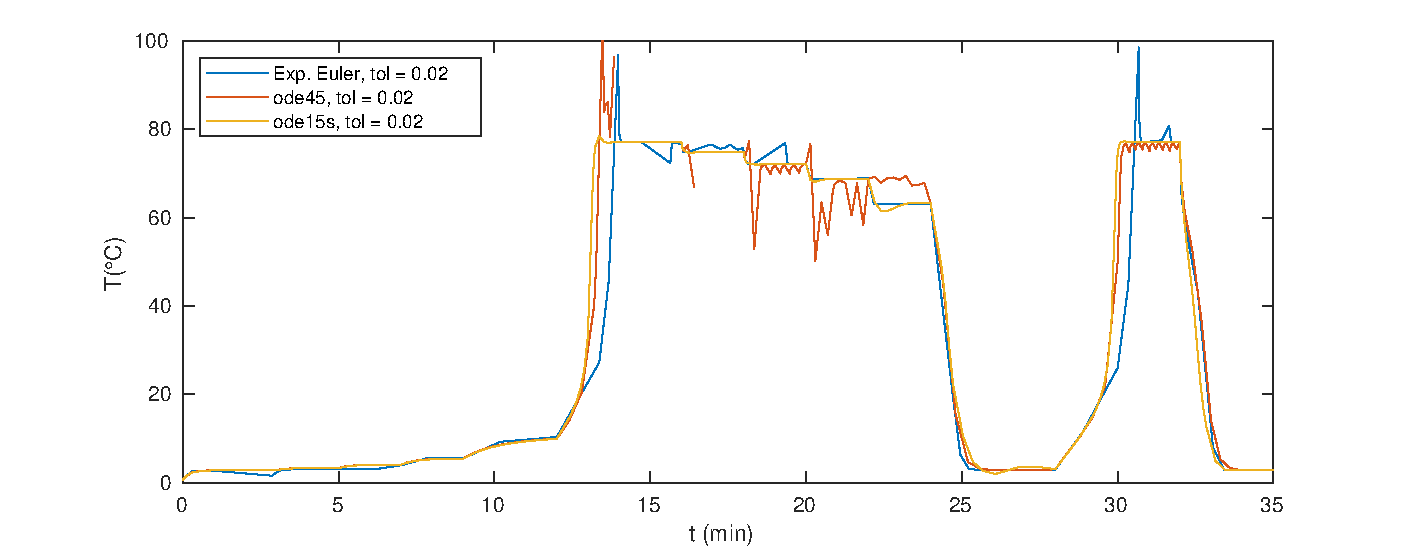
\includegraphics[width=1\linewidth]{images/2/2_6_1D.pdf}
        \caption{CSTR 1D problem}
    \end{subfigure}
    \caption{Solution for the CSTR problem using Explicit Euler vs. \code{ode45} and \code{ode15s}}
    \label{2_6_3D_1D}
\end{figure}

\begin{table}[H]
    \centering
    \begin{tabular}{@{}l|c|c|c@{}}
    \toprule
    \textbf{Method}      & \textbf{Expl. Euler} & \textbf{ode45} & \textbf{ode15s} \\
    Tolerances           & 0.02                 & 0.02           & 0.02            \\ \midrule
    Function evaluations & 291                  & 1477           & 480             \\
    Calculated steps     & 168                  & 1555           & 1423            \\
    Accepted steps       & 123                  & 211            & 203             \\
    Rejected steps       & 45                   & 33             & 27              \\ \bottomrule
    \end{tabular}
    \caption{Parameters of the Explicit Euler vs. \code{ode45} and \code{ode15s} for the CSTR-3D problem}
    \label{2_6_3D_table}
\end{table}

\begin{table}[H]
    \centering
    \begin{tabular}{@{}l|c|c|c@{}}
    \toprule
    \textbf{Method}      & \textbf{Expl. Euler} & \textbf{ode45} & \textbf{ode15s} \\
    Tolerances           & 0.02                 & 0.02           & 0.02            \\ \midrule
    Function evaluations & 201                  & 1297           & 375             \\
    Calculated steps     & 117                  & 1270           & 1275            \\
    Accepted steps       & 84                   & 195            & 180             \\
    Rejected steps       & 33                   & 19             & 27              \\ \bottomrule
    \end{tabular}
    \caption{Parameters of the Explicit Euler vs. \code{ode45} and \code{ode15s} for the CSTR-1D problem}
    \label{2_6_1D_table}
\end{table}
